\section{Anexos}
\begin{center}
\begin{tabular}{r|cr}
 \begin{tabular}{c}
{\large\bf\textsf{\ M\'etodos Num\'ericos\ }}\\ 
Segundo Cuatrimestre 2013\\
{\bf Trabajo Pr\'actico 2}
\end{tabular} &
\begin{tabular}{l @{}}
 \emph{Departamento de Computaci\'on} \\
 \emph{Facultad de Ciencias Exactas y Naturales} \\
 \emph{Universidad de Buenos Aires} \\
\end{tabular} 
\end{tabular}
\end{center}

\vskip 25pt
\hrule
\vskip 11pt
 
\textbf{Introducci\'on}

El Equipo de Consultor\'ia de M\'etodos Num\'ericos busca desarrollar un software que pueda ser utilizado durante el
proceso de construcci\'on de puentes, otorgando informaci\'on respecto de la seguridad y los costos involucrados que
faciliten la toma de decisiones durante el mismo. Como punto de partida, nos concentraremos en un tipo particular de
puentes, llamados \emph{Pratt Truss Bridges}.\\

Para realizar el an\'alisis, es posible simplificar el problema y realizar el an\'alisis de la estructura en dos
dimensiones suponiendo que el peso se distribuye de forma homog\'enea en la tercera dimensi\'on. El puente debe tener una determinada longitud (\emph{span}), altura (\emph{h}) y se divide en un n\'umero par
de secciones ($n$) de igual tama\~no. La estructura se representa mediante \emph{links} (que modelan los miembros de la estructura) y
juntas (puntos donde se unen los links). La Figura \ref{fig:structex} muestra un ejemplo del modelo para la estructura.
Las juntas son representadas mediante un circulo blanco y los links mediante una l\'inea recta.

\begin{figure}[!ht]
\begin{center}
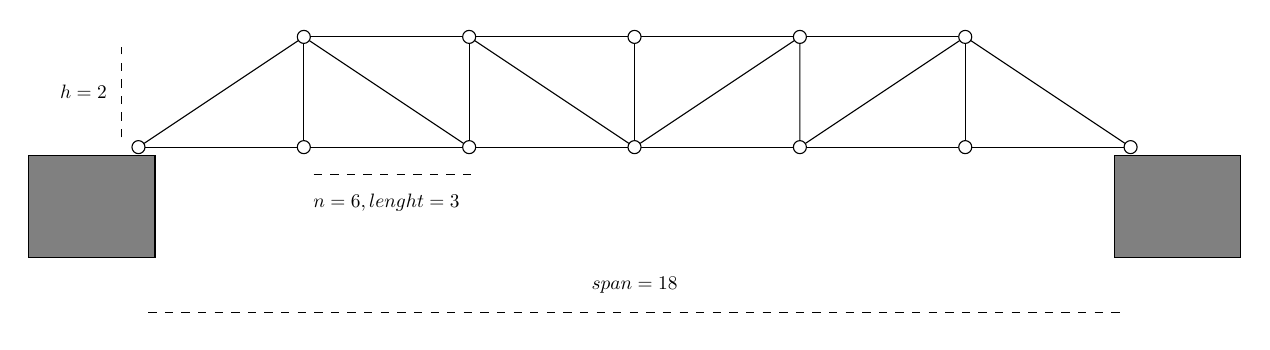
\begin{tikzpicture}[scale = 0.7]

    \tikzset{nodestyle/.style={draw,shape=circle,scale=0.5}}
    \node[nodestyle] (p1) at ( 0, 0) {}; 
    \node[nodestyle] (p2) at ( 3, 0) {};
    \node[nodestyle] (p3) at ( 6, 0) {};
    \node[nodestyle] (p4) at ( 9, 0) {};
    \node[nodestyle] (p5) at ( 12, 0) {};
    \node[nodestyle] (p6) at ( 15, 0) {};
    \node[nodestyle] (p7) at ( 18, 0) {};

    \node[nodestyle] (p8) at ( 3, 2) {};
    \node[nodestyle] (p9) at ( 6, 2) {};
    \node[nodestyle] (p10) at ( 9, 2) {};
    \node[nodestyle] (p11) at ( 12, 2) {};
    \node[nodestyle] (p12) at ( 15, 2) {};

    \begin{scope}[every path/.style={-}]
        \draw (p1) -- (p2);
        \draw (p2) -- (p3); 
        \draw (p3) -- (p4);
        \draw (p4) -- (p5);
        \draw (p5) -- (p6);
        \draw (p6) -- (p7);

        \draw (p8) -- (p9);
        \draw (p9) -- (p10);
        \draw (p10) -- (p11);
        \draw (p11) -- (p12);

        \draw (p1) -- (p8);
        \draw (p12) -- (p7);

        \draw (p2) -- (p8);
        \draw (p3) -- (p9);
        \draw (p4) -- (p10);
        \draw (p5) -- (p11);
        \draw (p6) -- (p12);

        \draw (p8) -- (p3);
        \draw (p9) -- (p4);
        \draw (p4) -- (p11);
        \draw (p5) -- (p12);
    \end{scope}  

        \draw[fill=gray] (0.3,-0.15) rectangle (-2,-2);
        \draw[fill=gray] (17.7,-0.15) rectangle (20,-2);

        % Nodos artificiales.
        \node (a1) at ( 0, -3) {};
        \node (a2) at ( 18, -3) {};
        \node (a3) at ( -0.3, 0) {};
        \node (a4) at ( -0.3, 2) {};
        \node (a5) at ( 3, -0.5) {};
        \node (a6) at ( 6.3, -0.5) {};
        \node[scale=0.7] (l1) at ( 9, -2.5) {$span = 18$};
        \node[scale=0.7] (l2) at ( -1, 1) {$h = 2$};
        \node[scale=0.7] (l2) at ( 4.5, -1) {$n = 6, lenght = 3$};
        
        \begin{scope}[every path/.style={-}]
            \draw[dashed] (a1) -- (a2) ;
            \draw[dashed] (a3) -- (a4) ;
            \draw[dashed] (a5) -- (a6) ;
        \end{scope}
        
\end{tikzpicture}
\caption{Ejemplo estructura en 2D}
\label{fig:structex}
\end{center}
\end{figure}

Para que la estructura del puente pueda ser utilizada, debe soportar una carga total (conocida) que se distribuye entre 
las juntas internas inferiores del puente. Este hecho afecta a toda la estructura del puente y por lo tanto los links
que conforman la misma deben ser lo suficientemente resistentes para mantener estable la estructura. El objetivo del
trabajo es realizar este an\'alisis para distintos tipos de estructuras.
